%\documentclass[iop]{emulateapj}
\documentclass[aps, prl, twocolumn, groupedaddress, amsfonts, amssymb, amsmath]{revtex4-1}
\usepackage{graphicx}
\usepackage{bm}
\usepackage{natbib}
%\usepackage[colorlinks=True, linkcolor=blue, citecolor=blue]{hyperref}
%\usepackage[all]{hypcap}

\bibliographystyle{apsrev}

\newcommand{\Div}[1]{\ensuremath{\nabla\cdot\left( #1\right)}}
\newcommand{\angles}[1]{\ensuremath{\left\langle #1 \right\rangle}}
\newcommand{\grad}{\ensuremath{\nabla}}
\newcommand{\RB}{Rayleigh-B\'{e}nard }
\newcommand{\stressT}{\ensuremath{\bm{\bar{\bar{\Pi}}}}}
\newcommand{\nrho}{\ensuremath{n_{\rho}}}


\begin{document}
%%%%% Create nice title and abstract
\author{Evan H. Anders}
\affiliation{Department of Astrophysical \& Planetary Sciences, University of Colorado -- Boulder}
\affiliation{Laboratory for Atmospheric and Space Physics, Boulder, CO}
\author{Benjamin P. Brown}
\affiliation{Department of Astrophysical \& Planetary Sciences, University of Colorado -- Boulder}
\affiliation{Laboratory for Atmospheric and Space Physics, Boulder, CO}
\title{Convective heat transport in stratified atmospheres at low and high Mach number}

\begin{abstract}
Here we study stratified convection in the context of polytropically stratified atmospheres. 
We hold the density stratification and Prandtl number (Pr) constant while studying the dependence
of the Nusselt number (Nu), which quantifies the efficiency of convective heat transport, on
variations of the Mach number (Ma) and the Rayleigh number (Ra).  In the low Ra regime, high and
low Ma flows have very different scalings of Nu with Ra.  In the high Ra regime, high and low Ma flows
have nearly the same scaling of Nu with Ra, with power laws near (enter here), reminiscent of the
Nu $\propto$ Ra$^{2/7}$ seen in \RB convection.
\end{abstract}
\maketitle


%%%%% Body of the paper
\section{Introduction}
\refstepcounter{section}
\label{sec:intro}
Convection is essential to heat transport in the cores of high mass stars, the
envelopes of low mass stars, and the atmospheres of terrestrial and jovian planets. In such systems, convection
occurs in the presence of the atmospheric stratification, which can be small but extends up to 
14 density scale heights in the Sun's convective envelope.
A basic understanding of the
properties of compressible convection in stratified media is important to understanding systems in astrophysics
and planetary sciences.  Numerical constraints typically have restricted studies of stratified convection to
moderately high Mach numbers, appropriate to regions near the Sun's surface.  As such, we know little about the
fundamental properties of low-Mach number stratified convection, which occurs in the deep solar interior.

Some of the earliest numerical experiments on stratified convection
were performed in two \cite{graham1975, chan&all1982,
hurlburt&all1984, cattaneo&all1990} and three \cite{cattaneo&all1991, brummell&all1996} dimensions and
revealed a number of basic properties in the moderate-to-high Mach number regime.
Unlike the widely-studied \RB problem, in which upflows and downflows are symmetrical, highly stratified
convection exhibits high-velocity, narrow downflow lanes and slow, broad upflow lanes.  As velocities approach
the speed of sound, shocks begin to form near the downflow lanes at the top of the atmosphere and propagate toward the upflows.
In \RB convection, the temperature gradient
and by proxy the radiative flux approach zero in the convecting region.  In stratified convection, the 
\emph{entropy} gradient is flattened by convection, but this does not necessitate the disappearance of the
radiative flux due to contributions of thermodynamic variables other than temperature to the entropy.

In \RB convection, there exist two primary control parameters: the Rayleigh number (Ra), the ratio of
buoyant driving to diffusive damping, and the Prandtl number (Pr), the ratio of viscous to thermal
diffusivity.  Along with the aspect ratio of the physical domain, these two numbers entirely control the
dynamics of the convection.  In stratified atmospheres, in addition to specifying the equation of state and
fundamental properties of the gas, the two control parameters of \RB convection are joined by the degree of
stratification across the domain and the characteristic Mach number (Ma) of the convective flows.  
Polytropically stratified atmospheres, such as those used in early studies, are an ideal extension of
\RB convection into the stratified realm as the two additional control parameters are directly linked to
basic properties of the atmosphere.  The density stratification is set by the number of density scale heights
the atmosphere spans (\nrho), and the Mach number is controlled by the superadiabatic excess ($\epsilon$),
which is the deviation of the polytropic index from that of an adiabatic polytropic index \cite{graham1975}.

In this letter, we study the effects of variations of $\epsilon$ and Ra on the heat transport of convection
in polytropically stratified atmospheres, characterized by the Nusselt number (Nu).  We hold \nrho and Pr
constant across all simulations and examine moderate (4) and large (8) aspect ratios.  In section 
\ref{sec:experiment}, we describe the construction of atmospheres, our equations, and our method for
numerical time evolution.  We describe our findings in section \ref{sec:results} and discuss
implications in section \ref{sec:discussion}.

\section{Experiment} 
\refstepcounter{section}
\label{sec:experiment}
In order to compare our results with previous studies and in an effort to examine a simplest case,
we study a fluid composed of monatomic ideal gas particles, with an adiabatic index of $\gamma = 5/3$ and
whose equation of state is $P = R^*\rho T$. 
The initial stratification is polytropic, such that the gravitational
acceleration and conductive heat flux are invariant throughout the depth of the atmosphere. In order
to satisfy the latter assumption, the thermal conductivity, $\kappa$ and temperature gradient
$\grad T_0$ are often taken as constants, such that $\bm{F}_{\text{cond,0}} = -\kappa \grad T_0 = \text{constant}$.
Under these assumptions, solving the equation of hydrostatic equilibrium produces an atmosphere defined by
\begin{equation}
\begin{split}
\rho_0(z) &= \rho_{00}(z_0 - z)^m \\
T_0(z)    &= T_{00}(z_0 - z),
\label{eqn:polytrope}
\end{split}
\end{equation}
where $z$ increases upwards within the bounds $z =\{0, L_{z}\}$.
We specify the number of density scale heights the atmosphere spans, $n_\rho$, to determine $L_{z}$. Throughout
this letter, we set $n_{\rho} = 3$ such that the density at the bottom of the atmosphere is larger
than at the top by a factor of 20.
Thermodynamic variables are nondimensionalized at the top of the atmosphere as 
$P_0(L_z) = \rho_0(L_z) = T_0(L_z) = 1$, requiring $z_0 \equiv L_z + 1$ and $R^* = T_{00} = \rho_{00} = 1$.  
The polytropic index is set by the adiabatic index and the
superadiabatic excess, $\epsilon$, such that $m = m_{ad} - \epsilon$
where $m_{ad} \equiv (\gamma-1)^{-1}$ is the adiabatic polytropic index.
The subsequent entropy gradient at the top of the atmosphere is $\grad S(L_z) = -\epsilon$,
the negative of the superadiabatic excess.  The characteristic timescale of such an
atmosphere is related to the characteristic atmospheric buoyancy time, $t_{\text{b}} = \sqrt{L_z/g\epsilon}$.
We will utilize buoyancy time units throughout this letter.

Atmospheric diffusivities are set by the Rayleigh number and the Prandtl number.  We define the
non-dimensional Rayleigh number as
\begin{equation}
\text{Ra} = \frac{g L_z^3 (\Delta S_0 / c_P)}{\nu\chi},
\end{equation}
where $\Delta S_0$ is the entropy difference between the top and bottom of the atmosphere, 
$\nu$ is the kinematic viscosity (viscous diffusivity), and $\chi$ is the thermal dififusivity.  
The relationship between the thermal and viscous diffusivities is
set by the Prandtl number, Pr$ = \nu/\chi$.   We relate the dynamic viscosity, $\mu$, and the thermal conductivity,
$\kappa$, to their corresponding diffusivities such that 
$\nu \equiv \mu/\rho$ and $\chi \equiv \kappa/\rho$.  As a result, $\text{Ra} \propto (\nu\chi)^{-1} \propto
\rho^2$, such that for our atmospheres with $n_{\rho} = 3$, the Rayleigh number increases by a factor of
400 from the top of the domain to the bottom of the domain.  Such a formulation leaves Pr
constant throughout the depth of the atmosphere, and in this letter we impose $\text{Pr} = 1$.

At the constant values of $n_\rho$ and Pr used, the primary control parameters of convection are $\epsilon$
and Ra.  We decompose our atmosphere into the background polytrope ($\ln\rho_{0}, T_{0}$) and the fluctuations
about that background ($\bm{u}, \ln\rho_{1}, T_{1}$).  The scaling of the entropy gradient with $\epsilon$
is reflected in the evolved values of these fluctuations, which follow the scaling of
Ma$^{1/2} \propto T_1/T_0 \propto \rho_{1}/\rho_{0} \propto \epsilon$, and which scale as roughly $Ra^{0.3}$,
as in Fig. \ref{fig:ma_v_eps}.

\begin{figure}[t]
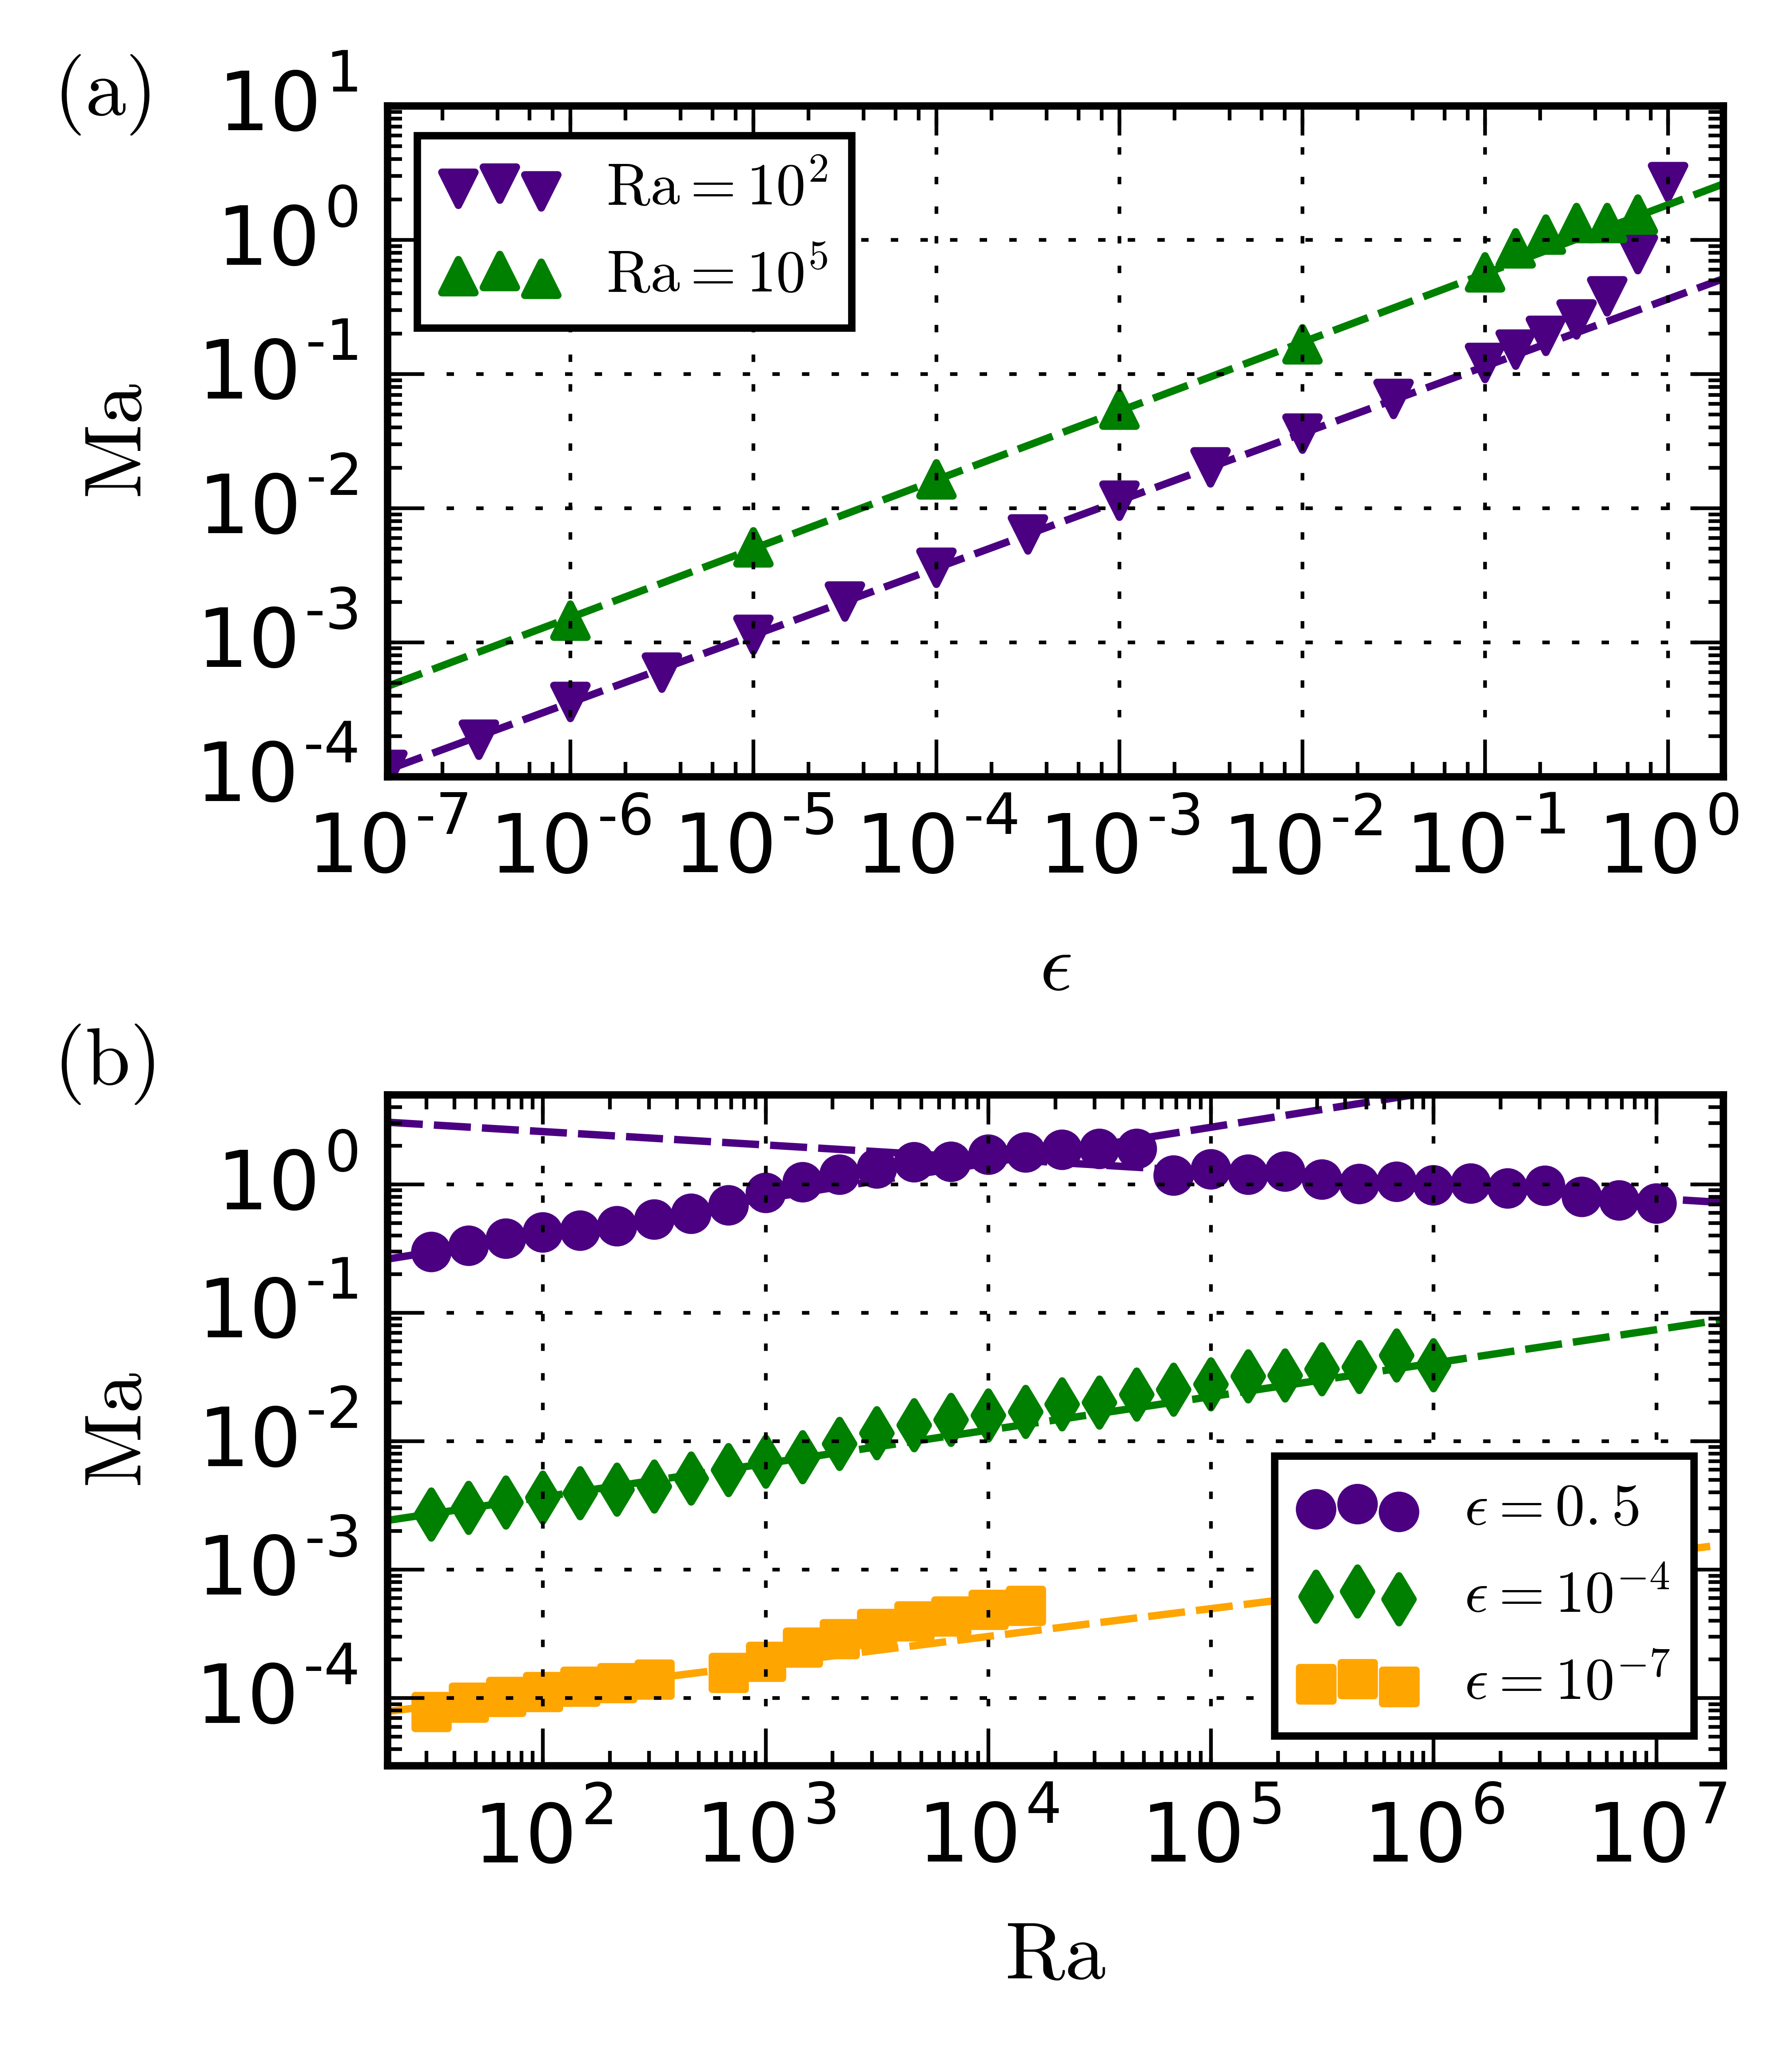
\includegraphics[width=3.4375in]{./figs/ma_v_eps.png}
\caption{(a) Characteristic horizontally averaged maximum Mach numbers which have been
time averaged over 100$t_{b}$ starting roughly 100$t_{b}$ after the start of simulations. At low $\epsilon$,
Ma shows power laws of $Ma \propto \epsilon^{0.5048}, \epsilon^{0.5129}$ at Ra = $10^2$ and $10^5$, respectively (need err bars).
When $\epsilon \rightarrow m_{ad}$, large deviations from this power law are seen and the system quickly
approaches Ma $\approx 1$.  Ma shows weak scaling with $\epsilon$, and does not exceed Ma$ \approx 1$
\label{fig:ma_v_eps} }
\end{figure}

We evolve the Fully Compressible Navier-Stokes equations,
which take the form:
\begin{align}
&\begin{aligned}
&\frac{D \ln\rho}{D t} + \Div{\bm{u}} = 0
	\label{eqn:continuity_eqn}
\end{aligned}\\
&\begin{aligned}
&\rho\frac{D\bm{u}}{D t}=
-\grad P + \rho\bm{g} - \nabla\cdot\stressT
	\label{eqn:momentum_eqn}
\end{aligned}\\
&\begin{aligned}
\rho c_V\left(\frac{D T}{D t} + (\gamma-1)T\Div{\bm{u}}\right) + &\Div{-\kappa\grad T} = \\
&-\left(\stressT\cdot\nabla\right)\cdot\bm{u} 
	\label{eqn:energy_eqn}
\end{aligned}
\end{align}
where $D/Dt \equiv \partial_t + \bm{u}\cdot\grad$ and the viscous stress tensor is defined as
\begin{equation}
\Pi_{ij} \equiv -\mu\left(\frac{\partial u_i}{\partial x_j} + \frac{\partial u_j}{\partial x_i} - \frac{2}{3}\delta_{ij}\Div{\bm{u}}\right).
	\label{eqn:stress_tensor}
\end{equation}

In such stratified systems, the total convective flux can be defined as
\begin{equation}
\bm{F}_{\text{conv}} \equiv \bm{F}_{\text{enth}} + \bm{F}_{\text{KE}} + \bm{F}_{\text{PE}} + \bm{F}_{\text{visc}},
\end{equation}
where $\bm{F}_{\text{enth}} \equiv \rho\bm{u}(c_V T + P/\rho)$ is the enthalpy flux, $\bm{F}_{\text{KE}} \equiv 
\rho|\bm{u}|^2\bm{u}$ is the kinetic energy flux, $\bm{F}_{\text{PE}} \equiv \rho\bm{u}\phi$ is the potential
energy flux (with $\phi \equiv -gz$), 
and $\bm{F}_{\text{visc}} \equiv \bm{u}\cdot\stressT$ is the viscous flux.  Taking an inner product of
Eq. \ref{eqn:momentum_eqn} with $\bm{u}$ and adding it to 
Eq. \ref{eqn:energy_eqn}, the full energy equation in conservation form is retrieved,
\begin{equation}
\frac{\partial}{\partial t}\left(\rho\left[\frac{|\bm{u}|^2}{2} + c_V T + \phi\right]\right) +
\Div{\bm{F}_{\text{conv}} + \bm{F}_{\text{rad}}} = 0
	\label{eqn:energy_eqn_full}
\end{equation}
where $\bm{F}_{\text{rad}} = -\kappa \grad T$.  An understanding of the flux terms is essential to characterizing
the convective heat transport in our systems.

The atmosphere is bounded above
and below by impenetrable, stress free, fixed temperature boundary conditions such that
\begin{equation}
w = \partial_z u = T_1 = 0
\end{equation}
at the boundaries. 


We utilize the novel Dedalus pseudospectral framework (cite website?) to time-evolve Eqs. 
\ref{eqn:continuity_eqn}-\ref{eqn:energy_eqn} using an implicit-explicit third-order four-step 
Runge-Kutta timestepping scheme \cite{ascher&all1997}.  
Variables are time-evolved on a dealiased Chebyshev (vertical)
and Fourier (horizontal, periodic) domain in which the
physical grid dimensions are 3/2 the size of the coefficient grid.  Our physical grid sizes range from
96x384 grid points at the lowest values of Ra to 1152x4608 grid points at Ra $\geq 10^{7}$. 
By using IMEX timestepping, we are able to study flows at moderate ($Ma \approx 1$) and very low ($Ma \approx 10^{-4}$)
Mach number (Fig. \ref{fig:ma_v_eps}b).

\section{Results}
\refstepcounter{section}
\label{sec:results}

The efficiency of convection is quantified by the Nusselt number.  
While the Nusselt number is well-defined in \RB convection
as the amount of total flux divided by the steady-state background conductive flux 
\cite{johnston&doering2009, otero&all2002},
a well-defined Nusselt number is more elusive in stratified convection.  A traditional definition of the Nusselt
number in stratified convection is \cite{graham1975,hurlburt&all1984}
\begin{equation}
N \equiv \frac{F_{\text{conv, z}} + F_{\text{rad, z}} - F_A}{F_{\text{ref}} - F_A},
\label{eqn:nusselt}
\end{equation}
where $F_{\text{conv, z}}$ and $F_{\text{rad, z}}$ are the z-components of $\bm{F}_{\text{conv}}$ and $\bm{F}_{\text{rad}}$,
respectively.  $F_A$ is the adiabatic conductive flux, defined as $F_A = -\kappa \partial_z T_{\text{ad}}$.  For an
atmosphere in hydrostatic equilibrium, such as a polytrope, $\partial_z T_{\text{ad}} \equiv - g / c_{P}$, and thus
$F_A = \kappa g / c_{P}$.  $F_{\text{ref}} = \Delta T / L_z$ is the conductive flux of a linear profile connecting the upper
and lower plates, where $\Delta T = T_{u} - T_{\ell}$.  

We contend that this is the general form of the Nusselt number.  To illustrate this, we consider a few limiting
cases. Convection works to
suppress entropy stratification and create isentropic atmospheres.  Under the Boussinesq approximation where
density variations are ignored, entropy stratification is directly proportional to temperature stratification,
such that $\grad S \rightarrow 0$ only when $\grad T \rightarrow 0$.  Thus, for \RB convection, 
$\grad T_{\text{ad}} \equiv 0$ and the familiar form of $N$ is retrieved.  In the case of stratified convection,
as $\epsilon \rightarrow m_{ad} + 1$, $\grad P \propto g \rightarrow 0$ and
the resulting $\grad T_{\text{ad}} \rightarrow 0$.  In such a case, $F_A \rightarrow 0$ and the familiar
definition of the \RB nusselt number is appropriate to use, which explains why convection carries all of the
atmosphereic flux in such a case \cite{brandenburg&all2005}. As $\epsilon \rightarrow 0$, 
$\grad T_{\text{ad}}\rightarrow \grad T_0$, the atmospheric initial temperature profile.  This causes increasingly
smaller velocity, temperature, and pressure perturbations (e.g. Fig. \ref{fig:ma_v_eps}), but due to the removal
of the background radiative flux from the numerator and denominator in Eq. \ref{eqn:nusselt}, increasingly smaller
perturbations have just as large of an effect on the nusselt number.

We solved initial value problems which start in hydrostatic and thermal equilibrium and experienced infinitesimal 
kicks compared to $\epsilon$ in $T_1$.  Solutions were time-evolved until a long-time average of $N$ showed little
dependence on height. At
high values of $\epsilon$, shock systems form in the upper atmosphere near downflow lanes 
(see e.g. Fig. \ref{fig:entropy_snapshots}a) and propagate towards upflow lanes.  Such systems were reported in
both two \cite{cattaneo&all1990} and three \cite{malagoli&all1990} dimensional polytropic simulations previously.
Low mach number flows, such as those in an $\epsilon = 10^{-4}$ atmosphere (e.g. Fig. \ref{fig:entropy_snapshots}b)
have similar bulk thermodynamic structure but lack the complicating dynamics of shock heating. As Ra is
increased to very large values (e.g. Fig. \ref{fig:entropy_snapshots}c), thermodynamic structures no longer span
the vertical extent of the domain but instead break up into small packets which traverse through the domain many
times before diffusing.  The complicated nature of high Ra dynamics, especially in the low Ma regime where
shocks are absent, has barred us from sufficiently converging any solutions in the regime of $Ra > 10^7$.

\begin{figure}[t]
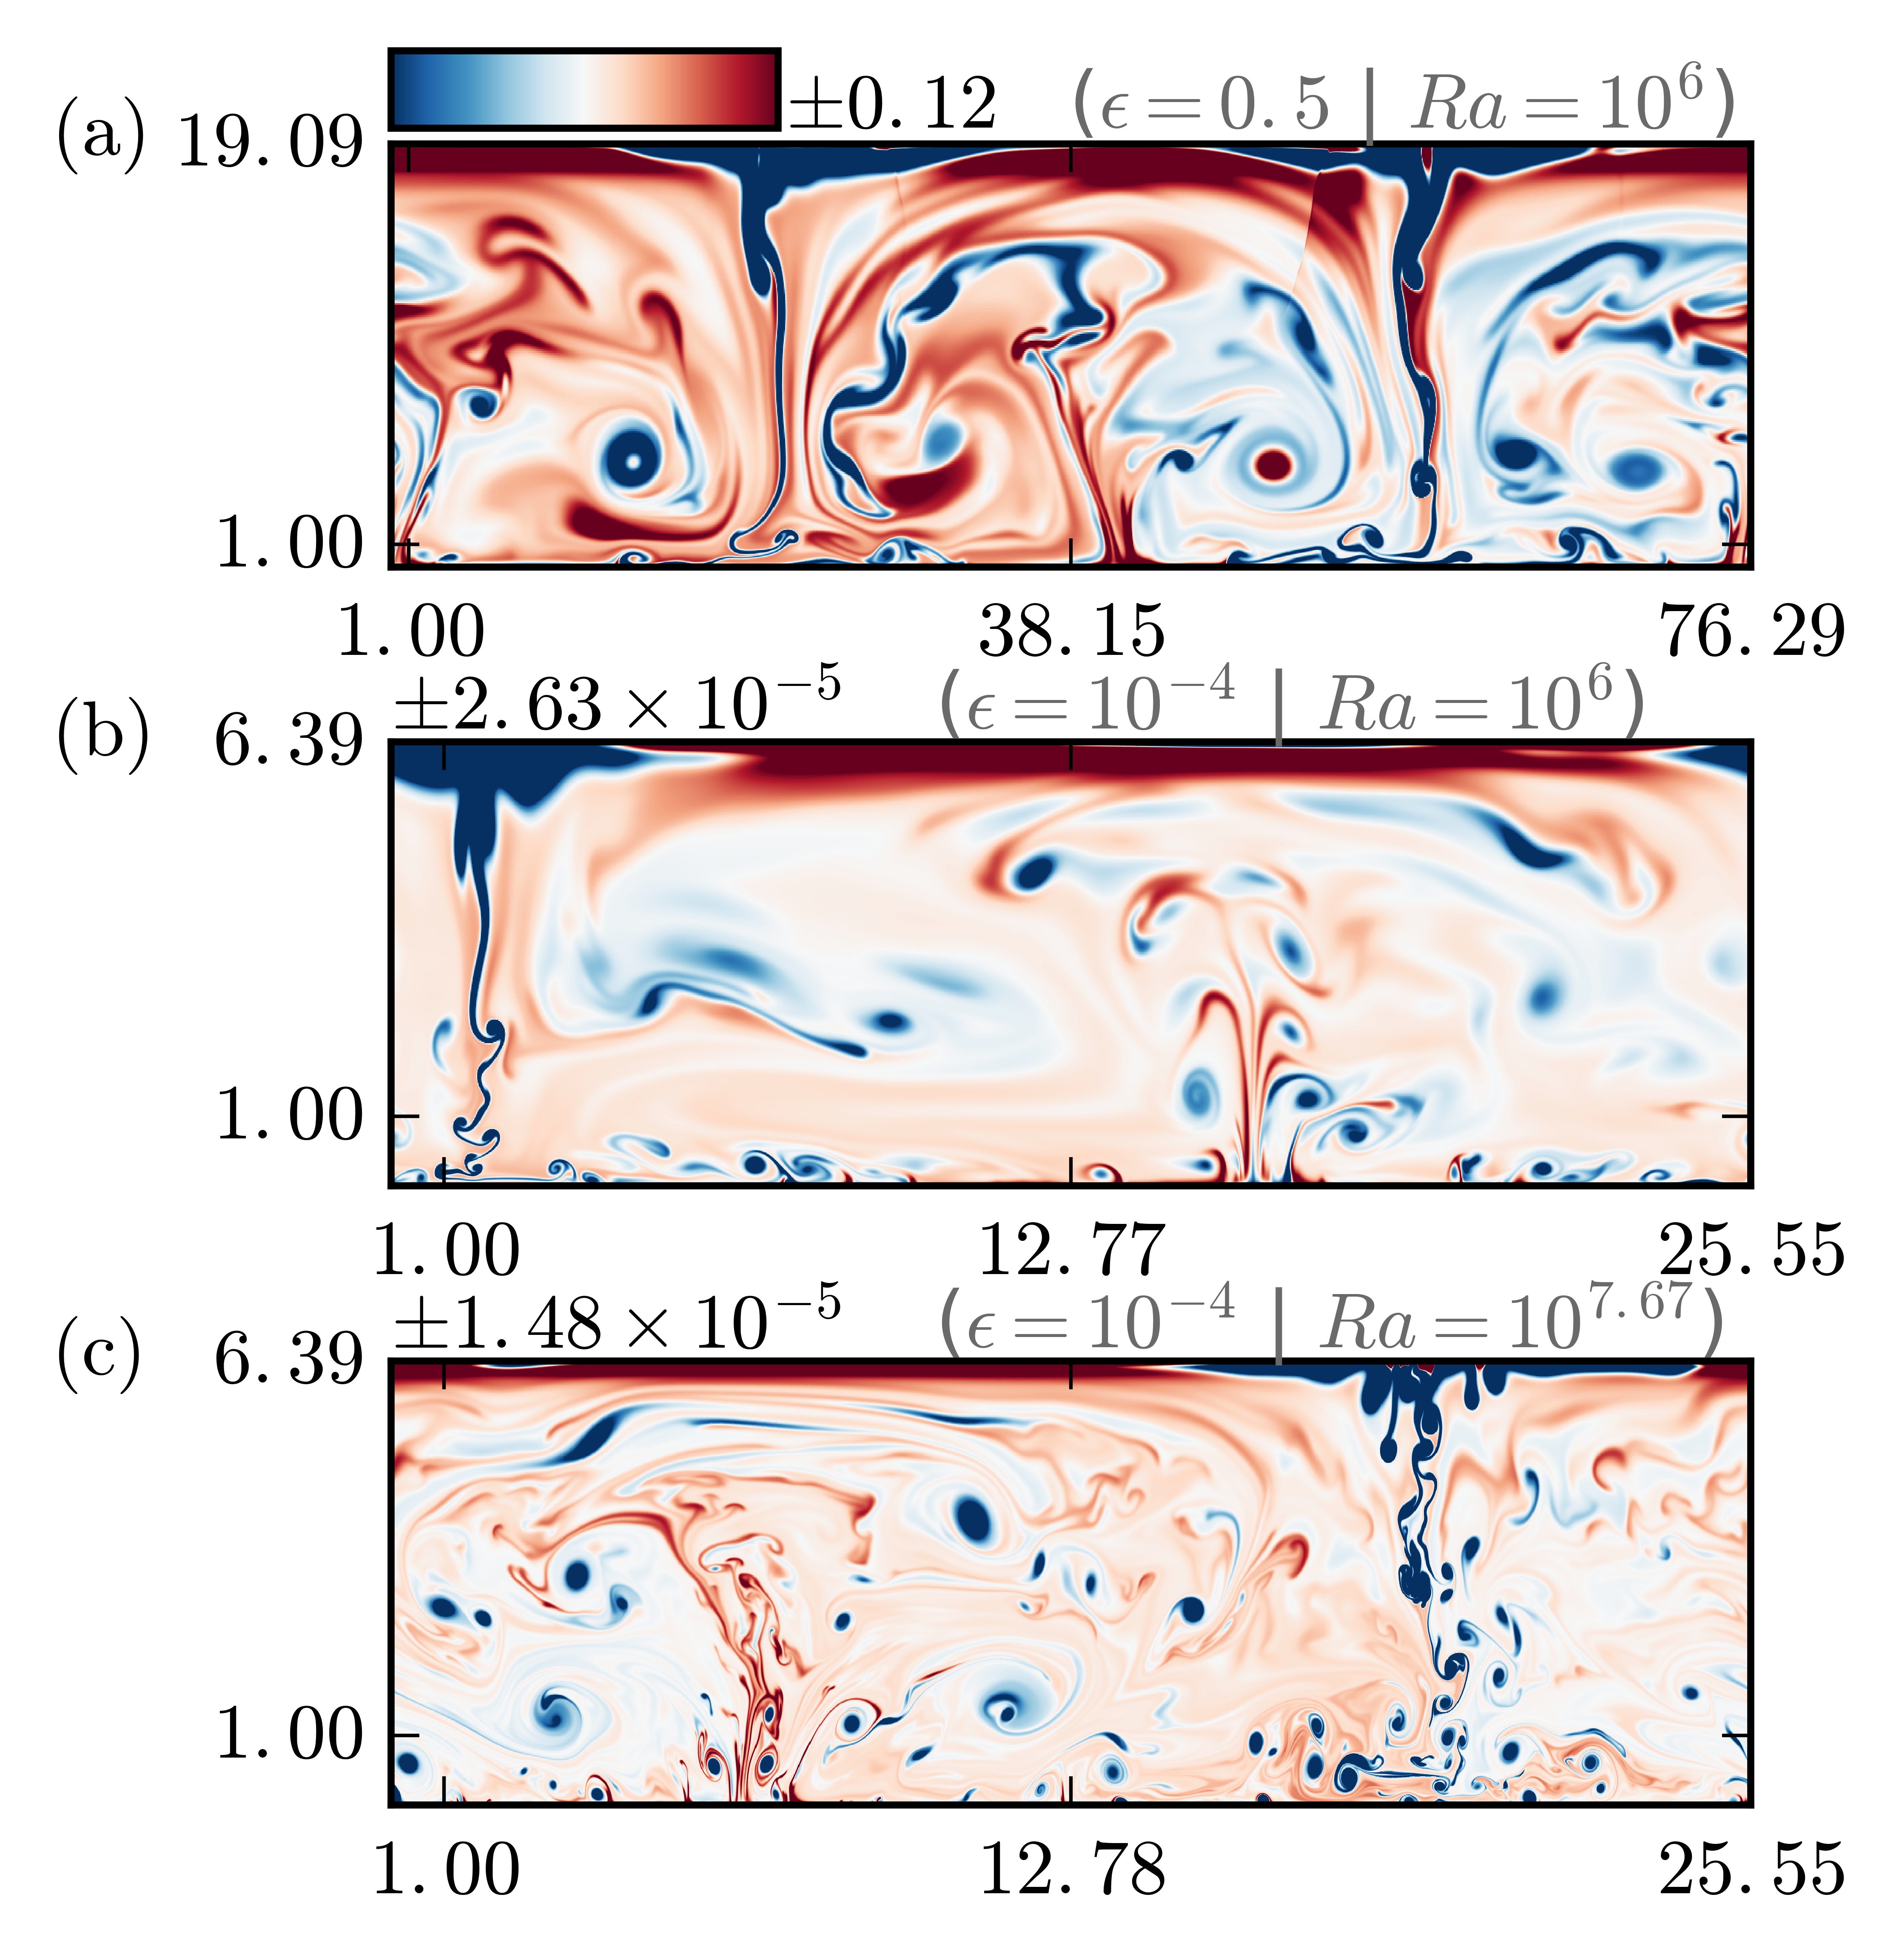
\includegraphics[width=3.4375in]{./figs/snapshots_fig.png}
\caption{Characteristic entropy. The time- and horizontally-
averaged profile is removed in all cases.  At high
$\epsilon$ (a), shock systems form near the upper downflow lanes and propel shock-heated material deep within
the atmosphere at sufficiently high Ra.  At low $\epsilon$ but at the same Ra (b), shock systems are absent, 
but otherwise the dynamics are similar.  As Ra is increased (c), downflow lanes no longer span
the entirety of the domain and individual cold, small blobs are responsible for carrying the flux downward.
\label{fig:entropy_snapshots} }
\end{figure}


Despite diferent thermodynamic structures, the properly normalized \emph{sum} of the fluxes for a given
Ra is similar.  See, for example, Fig. \ref{fig:flux_profiles} to see time-averaged horizontal profiles of
the vertical system fluxes.  At high $\epsilon$ and Ra, $\bm{F}_{\text{enth}}$ and $\bm{F}_{\text{KE}}$
exhibit two local maxima over the depth of the domain, whereas at low $\epsilon$ and low Ma, there is only
one local maximum near the bottom of the domain.  Viscous fluxes become important near the bottom boundary
layer, and radiative flux is nearly zero everywhere in the domain except for near the boundaries where the
fixed-temperature boundary conditions create large deviations in $\grad T$ away from $\grad T_{\text{ad}}$.

\begin{figure}[t]
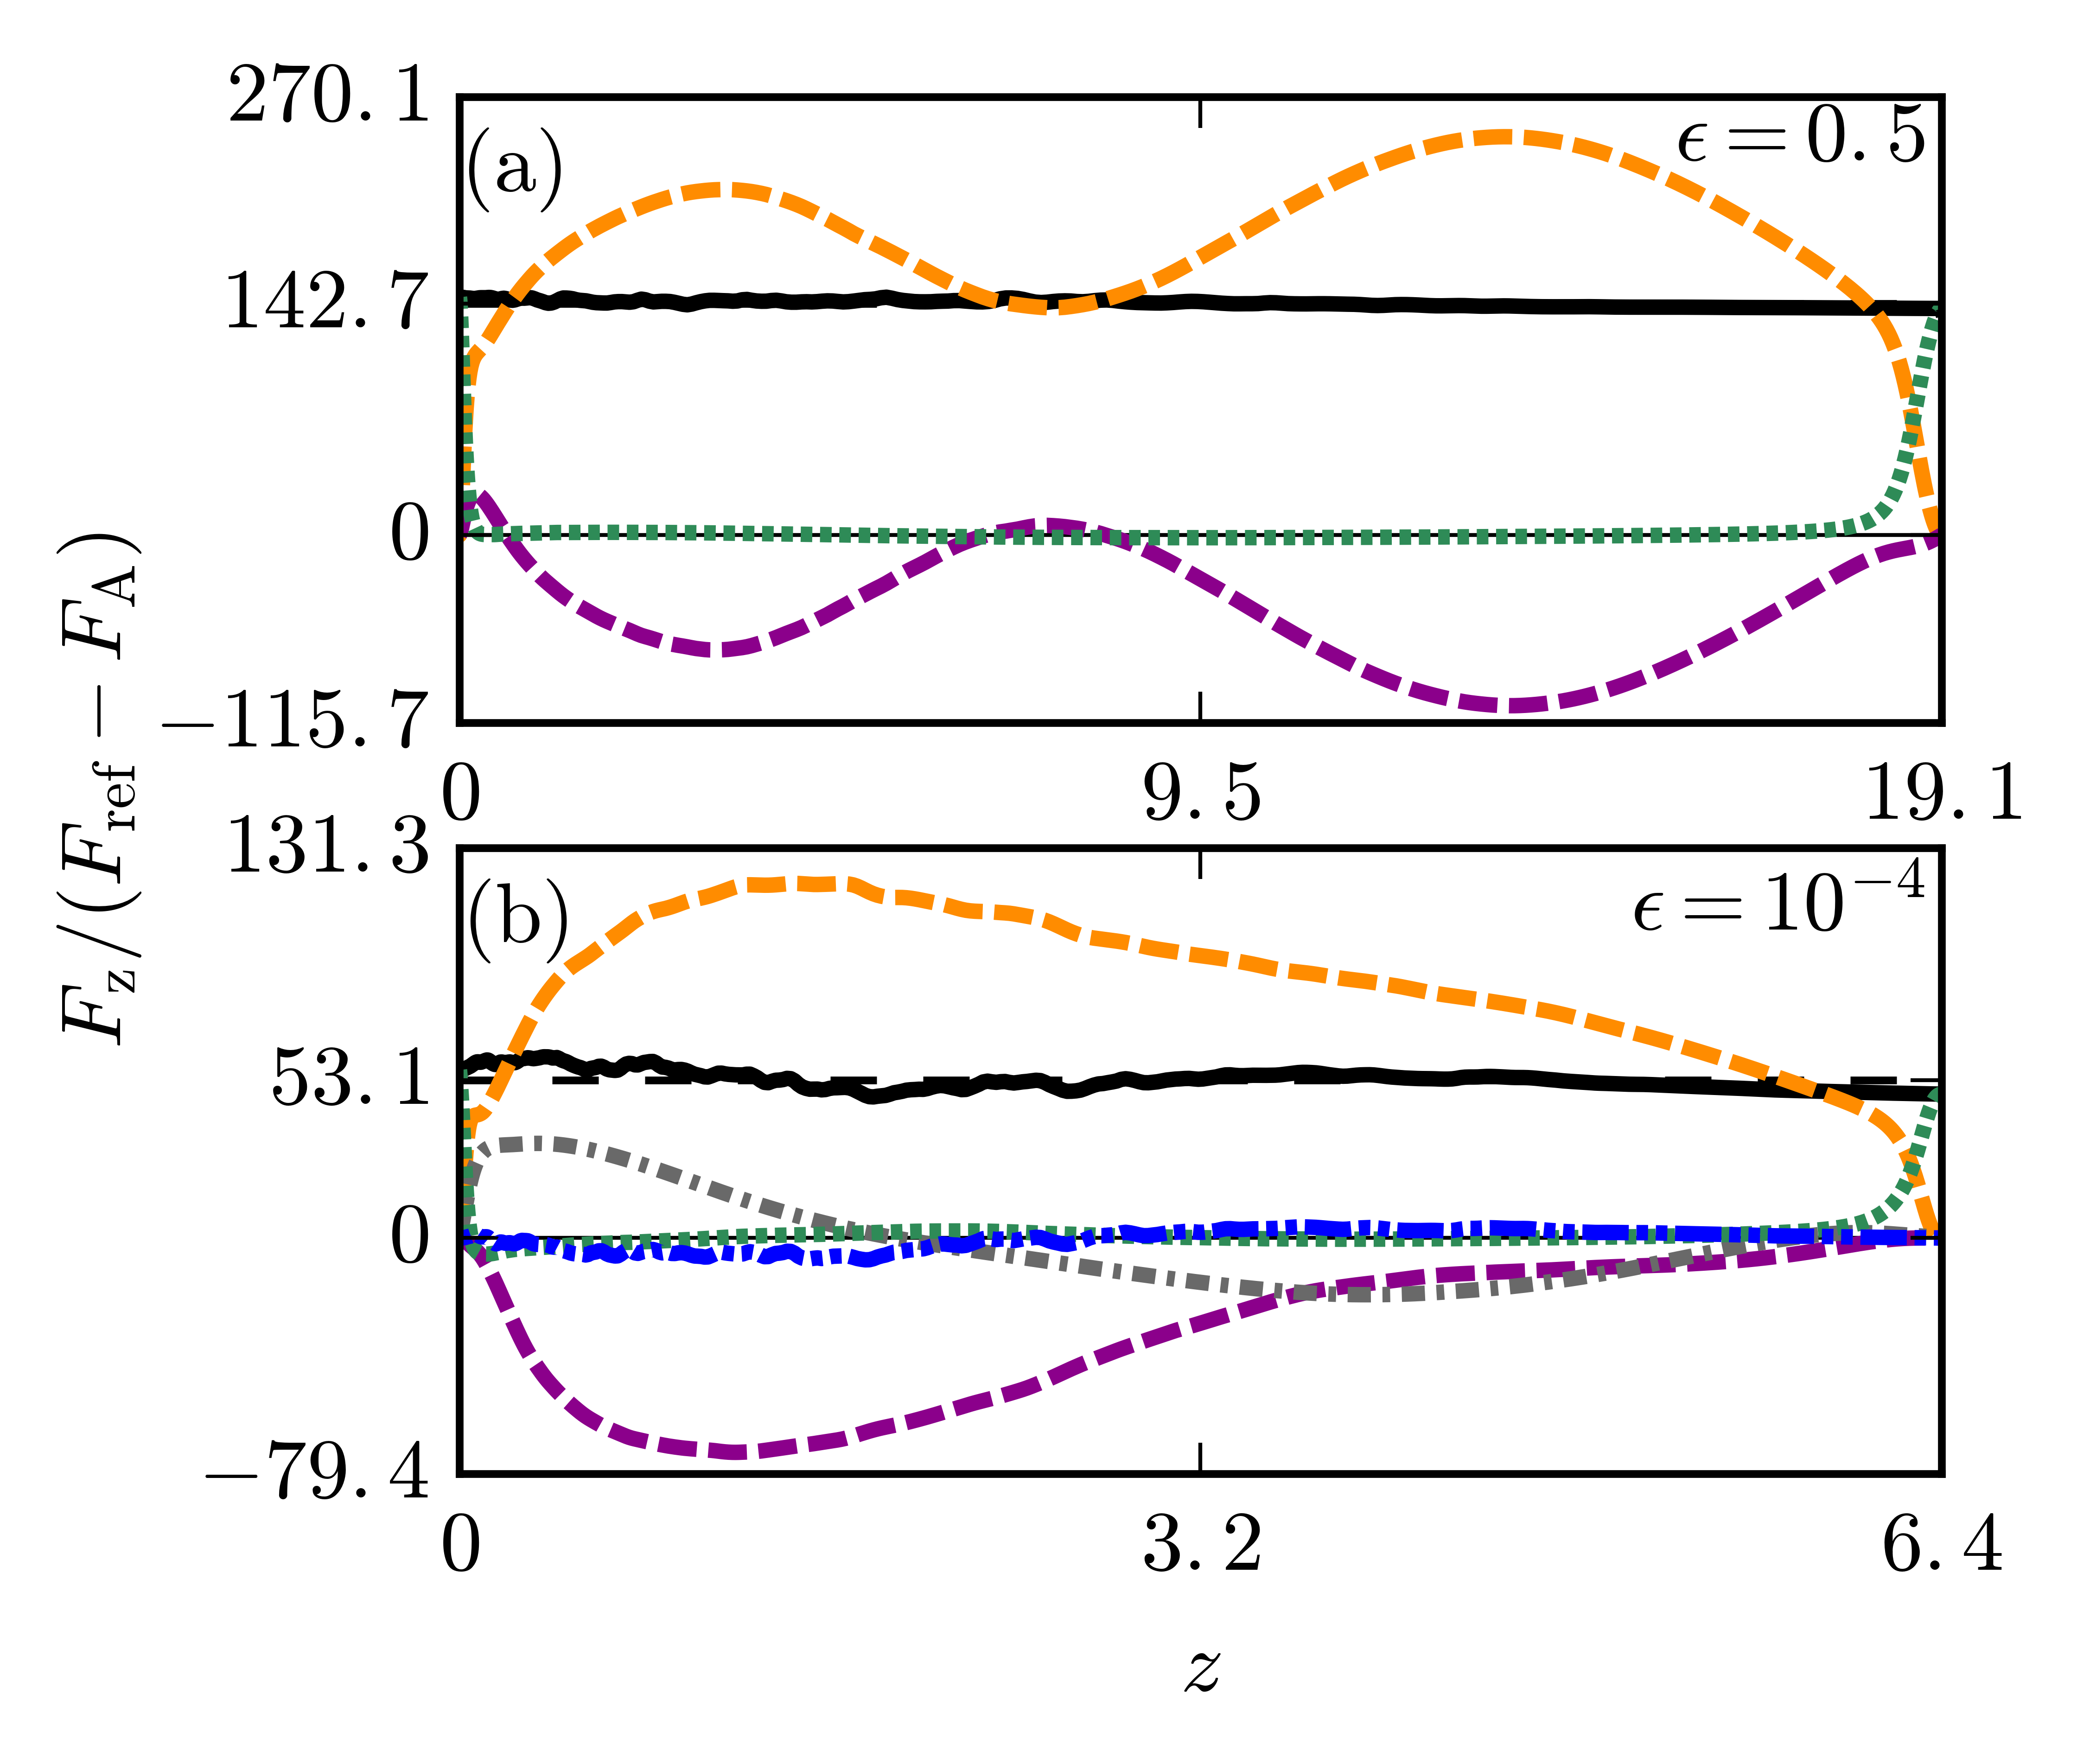
\includegraphics[width=3.4375in]{./figs/fluxes_fig.png}
\caption{Flux profiles for low (top) and high (bottom) Mach number flows.  
\label{fig:flux_profiles} }
\end{figure}

At low Rayleigh number, diffusivities are high and the flows are very laminar.  Such flows often achieve a
steady state and have a well-defined Nusselt number which is independent of time.  However, as the Rayleigh
number increases, the flows become increasingly time-dependent.  Even steady structures such as solid
``rolls'' like those pictured in Fig. \ref{fig:entropy_snapshots} have highly time-dependent Nusselt numbers.
This is, in part, due to the fact that cold downdrafts floating to the bottom of the domain can be entrained
by upflows, or warm risen parcels can be entrainedi n the intense cold downdrafts.  Such events reverse the
preferred direction of flux in the system, and even let the Nusselt number become negative for short periods of
time.  As a result, it is necessary to take a long time average of the fluxes
before calculating the Nusselt number at higher Rayleigh number. (IS THIS USEFUL?)

%
%\begin{figure}[t]
%\includegraphics[width=3.4375in]{./figs/nu_v_time.png}
%\caption{The evolution of the Nusselt number is shown at low ($10^2$) and high ($10^7$) Rayleigh number and at
%$\epsilon = 10^{-4}$.  At low Rayleigh number, the system is able to settle into a time invariant solution. As
%the Rayleigh number is raised, the thermodynamic structure become increasingly complex and time variant, and a
%time-average of the Nusselt number is required to obtain a sensible mean.
%\label{fig:nu_v_time} }
%\end{figure}

The evolution of the Nusselt number as the Rayleigh number is increased is shown for both high and low
$\epsilon$ in Fig. \ref{fig:nu_v_ra}.  Below convective onset, the Nusselt number is perfectly one. Just above
onset, there is a brief range of highly inflated scaling between $N$ and Ra. 

\begin{figure}[t]
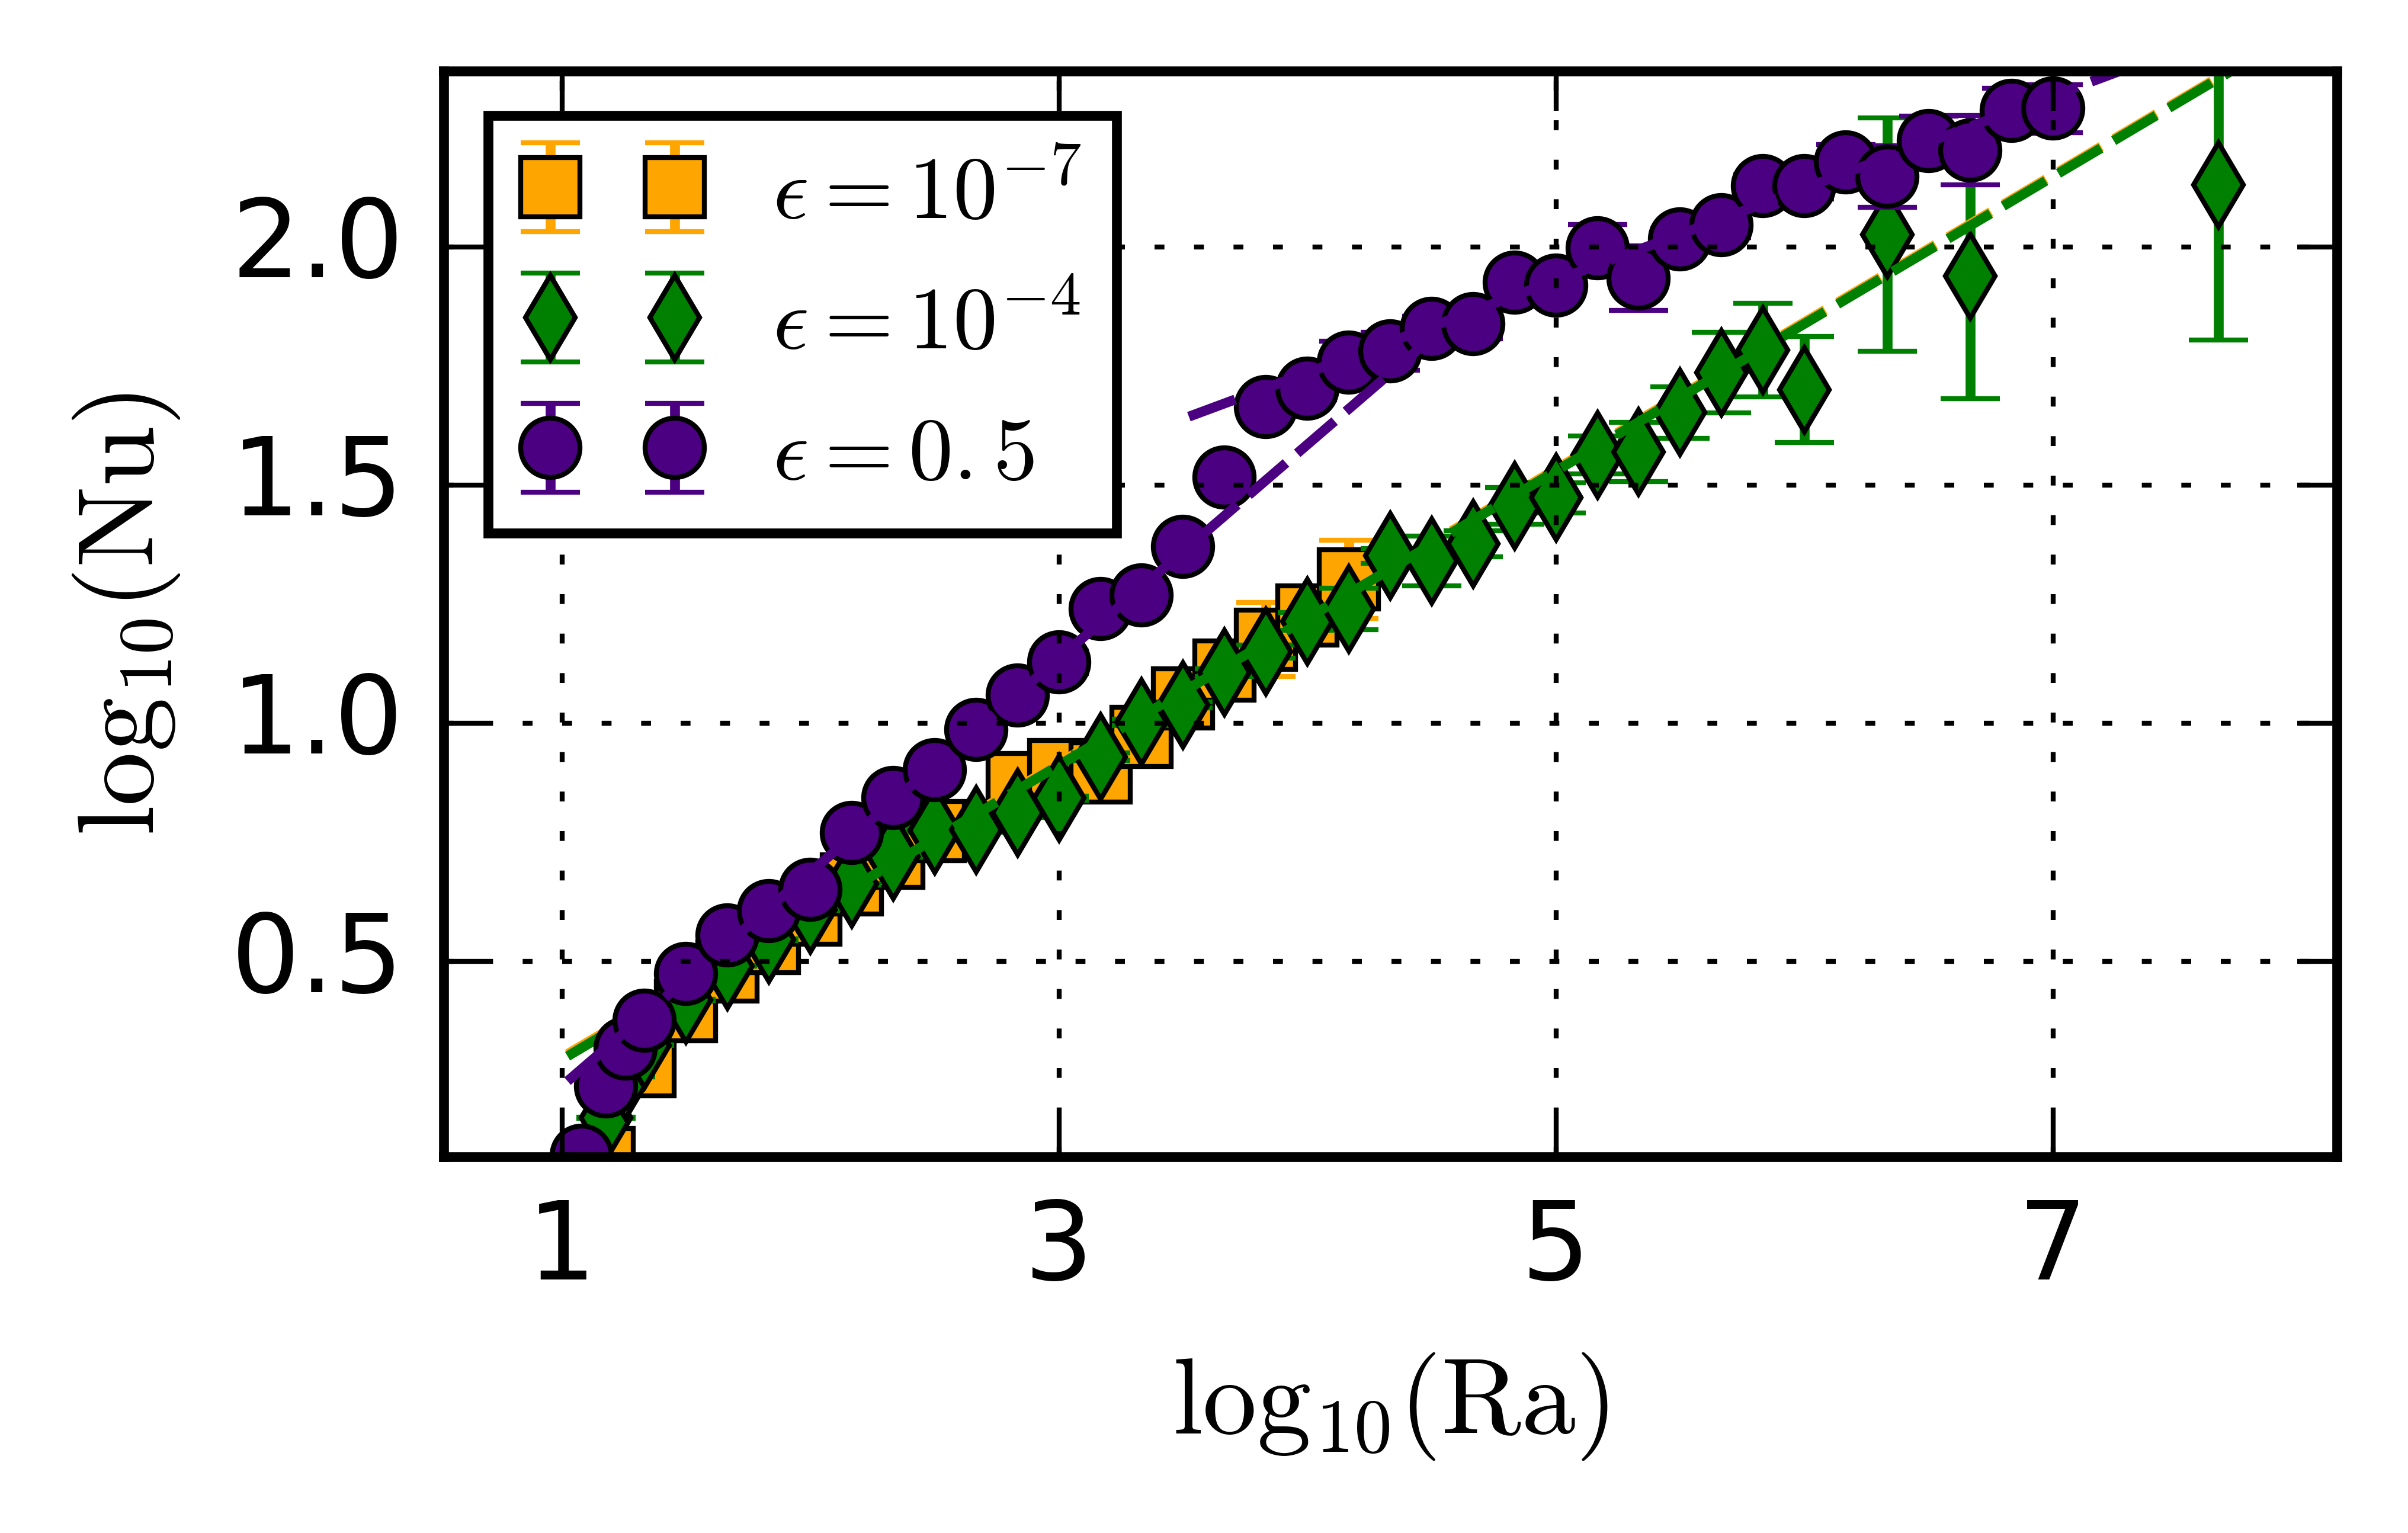
\includegraphics[width=3.4375in]{./figs/nu_v_ra.png}
\caption{Variation of the Nusselt number as a function of the Rayleigh number is shown.
\label{fig:nu_v_ra} }
\end{figure}

\section{Discussion}
\refstepcounter{section}
\label{sec:discussion}


\subsection{acknowledgements}
This work was supported by the CU/NSO Hale Graduate Fellowship and Juri's allocation and Ben's allocation.
We thank Axel Brandenburg, Mark Rast, and Jeff Oishi for many useful discussions.

\bibliography{../biblio.bib}
\end{document}
